\chapter{Simulação}\label{simula}

\section{O modelo proposto}

A figura a seguir ilustra essa metodologia descrita graficamente, onde as três etapas.

\pagebreak

\begin{figure}[ht]
\centering
\caption{Etapas da modelo proposto}
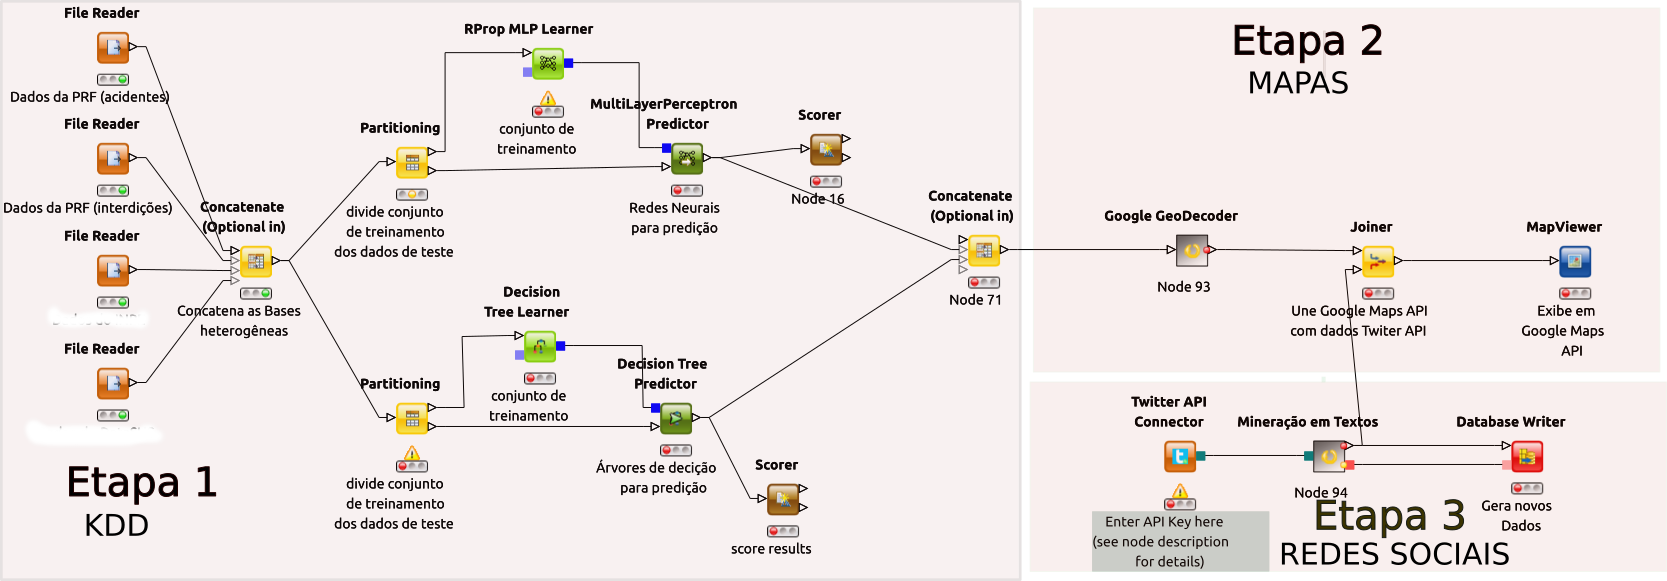
\includegraphics[width=170mm, height=85mm]{Figuras/Cronograma/metodologia.png}\\
\tiny Fonte: autor
\end{figure}

A \textbf{etapa 1} contempla a fases da coleta das bases de dados históricas, preparação dos dados e construção das variáveis do modelo preditivo.
  \begin{enumerate}
    \item O modelo preditivo integra várias bases de dados, tais como: Polícia Rodoviária Federal -- PRF, Batalhão de Polícia de Transito -- BPRv e dados históricos 
	   do Instituto de Pesquisas Espaciais -- INPE ou dos dados de precipitações pluviométricas do ``European Centre for Medium-Range Weather -- ECMWF.
 
    \item Algumas dessas informações também estão disponíveis em base de dados abertas, como sugere o Portal da Transparência, nos servidores da PRF além de outras
	  informações para complementar o sistema estão disponíveis na Internet sendo atualizadas pela PRF através de uma API aberta, esta pode 
	  ser configurável para se ligar ao nosso sistema.
    \item A conclusão dessa etapa ocorre com a Mineração dos dados e a extração de conhecimento.
	  Os ''outputs`` dessa etapa consiste em transformar os dados provenientes da mineração em coordenadas geográficas. 
	  As coordenadas geográficas são agrupadas a priori formando ''cluster`` de dados a serem exibidos em mapas vetoriais.\\
\end{enumerate}
  
A \textbf{segunda} etapa da metodologia contempla:
 \begin{enumerate}
    \item A malha viária representada em mapas de bases vetoriais;
    \item Um ambiente de simulação interativa que utiliza uma plataforma baseada na API do Google Maps.
  \end{enumerate}

A \textbf{terceira} e última etapa consiste em um módulo com as seguintes características:
  \begin{enumerate}
     \item Um módulo dinâmico onde são capturados ``feeds'' de redes sociais, por exemplo pelo Twitter. 
	Essa técnica faz um arco cibernético mantendo o sistema atualizado de informações.
     \item Através de um interligação a um banco de dados, esses ``feeds'' poderão ser usados para futuras predições.
  \end{enumerate}


\pagebreak


\section{A construção do Modelo preditivo}

O modelo preditivo foi construído utilizando bases de dados históricas da PRF (de acidentes e de paralisações ex: protestos) entre Janeiro de 2007 a 
Dezembro 2015. As bases de dados do Batalhão de Polícia de Rodoviária estadual -- BPRv vieram entre Janeiro/2010 a Julho/2016, cortes em ambas as bases foram 
feitos para adequar as datas. Essas bases de dados são integradas gerando um único e complexo modelo preditivo que será acoplado a estrutura dinâmica.


\subsection{Entendo e validando os dados de entrada -- input}
O segunda fase do ciclo CRISP-DM sugere uma análise para entendimento dos dados.
Na base de acidentes da PRF tentaremos traçar o perfil do condutor das BRs que atravessam o estado de Pernambuco.
Alguns gráfico do tipo histograma fornece uma análise explicativa desses dados de forma clara.
Na abcissa dos próximos gráficos estão os atributos mais relevantes das causas dos acidentes, elencamos os principais:
\begin{itemize}
 \item Condição da Pista: {Seca, Com burados, Molhada, Em obras, Com material granulado, Oleosa, Enlameada, Com gelo, Outras}
 \item Restrição de visibilidade: {Inexistente, Veículo Estacionado, Poeira/Fumaça/neblina, Vegetação, Ofuscamento, Cartazes/faixas, Placas}
 \item Traçado da via: {Reta, Curva, Cruzamento, Defeito}
 \item Tipo de veículo: {Automóvel, Caminhoneta, Motocicletas, Caminhão, Caminhão-trator, Bicicleta, Caminhonete, Ônibus, Motoneta, Micro-ônibus, Trator
 de rodas, Carroça, Caminhão-Tanque, Semi-Reboque, Utilitário, Ciclomotor, Charrete, Carro-de-mão, Quadriciclo, Trator misto, Reboque, Trator de esteiras,
 Não informado, Não se aplica, Não identificado}
\end{itemize}

%++++++++++++++++++++++++++++++++++++++++++++++++++++++++++++++++++++++++++++++++++++++++++++++
\subsection{Base da PRF -- acidentes}

\begin{figure}[ht]
\begin{center}
\caption{Condição Pista X Num. Acidentes -- Restrição visibilidade X Num. Acidentes}
\subfigure[Condição da Pista: Seca]{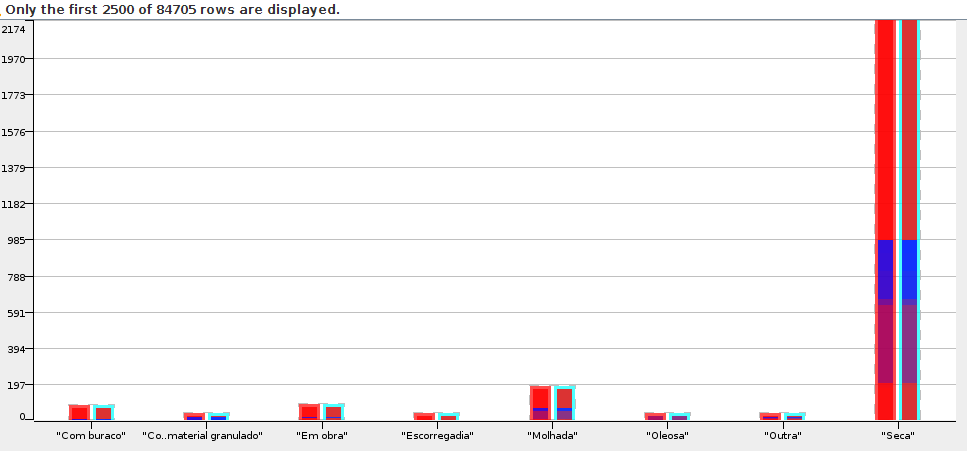
\includegraphics[width=75mm, height=48mm]{Figuras/Preprocess/CondicaoPistaXNumAcidentes.png}}
\qquad
%\caption{Restrição visibilidade X Num. Acidentes}
\subfigure[Restrição de visibilidade: Inexistente]{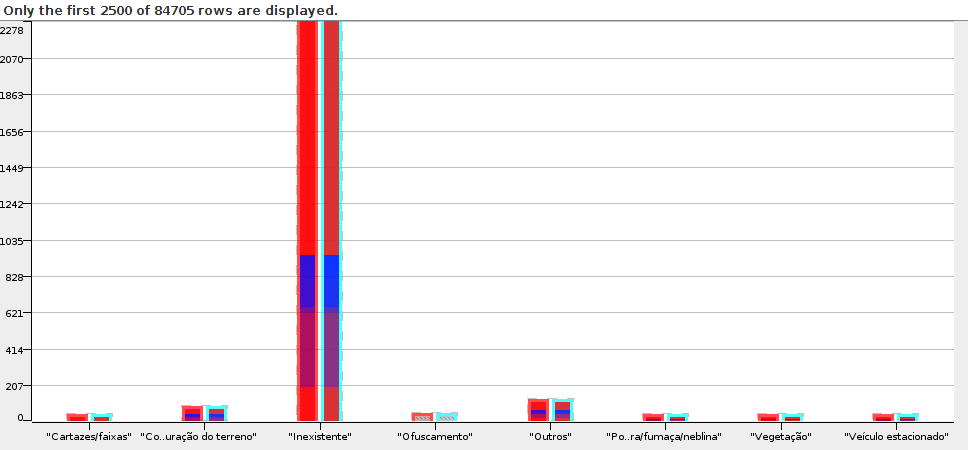
\includegraphics[width=75mm, height=48mm]{Figuras/Preprocess//RestricaoVisibilXBr.png}}\\
\tiny Fonte: autor
\end{center}
\end{figure}

A grande maioria dos acidentes ocorre com pista seca, sem restrição de visibilidade. 
A cor vermelha é referente a BR 101, a cor azul à BR 232, seguido das outras menos significativas.

\pagebreak

\begin{figure}[ht]
\begin{center}
\caption{Tipo de Veículo X Num. Acidentes}
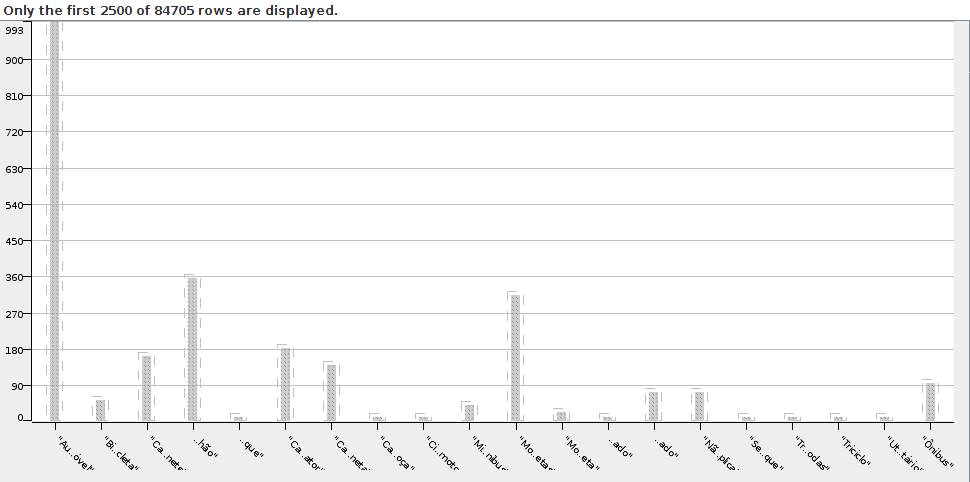
\includegraphics[width=150mm, height=80mm]{Figuras/Preprocess/TipoVeiculoXNumAciden.png}\\
\tiny Fonte: autor
\end{center}
\end{figure}

O maior número de acidentes ocorre com Automóvel de passeio, provavelmente condutores comuns, não profissionalizados.
O Caminhão é o segundo veículo que mais se envolve em acidentes, seguido das motonetas. 
Esses dados são referentes ao período entre 2007 à 2015.

\begin{figure}[ht]
\begin{center}
\caption{Traçado da via X Num. Acidentes}
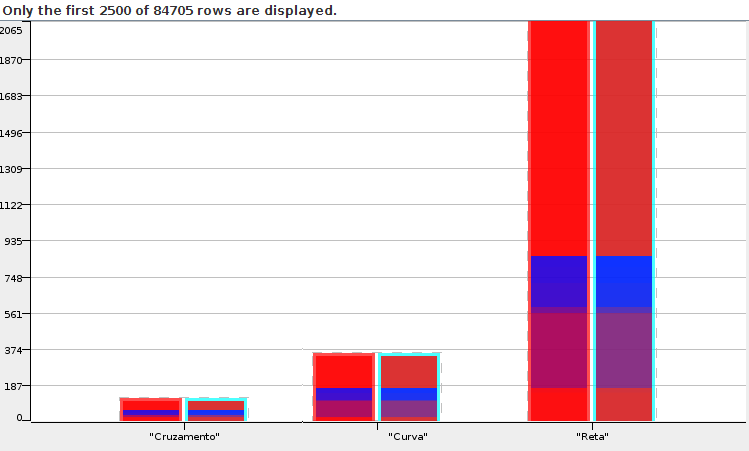
\includegraphics[width=120mm, height=70mm]{Figuras/Preprocess/TracadoViaNumAcident.png}\\
\tiny Fonte: autor
\end{center}
\end{figure}

O tipo de traçado da via não influência nas estatísticos de acidenes, pois a grande maioria dos acidentes ocorre em linha reta.
Esse comportamento do condutor nos faz crer o condutor é o responsável pelo maior número de ocorrências nas BRs.
Isso direciona nossa pesquisa para analisar e antever o comportamento do condutor, as condições da rodovia e ambientais nessa base
de dados não são fatores relevantes.

\pagebreak

\subsection{Base da PRF -- interdições}

\subsection{Base do IBGE}

\subsection{DataSUS}


\section{ As variáveis do modelo preditivo}

Algumas técnicas de IA são altamente sensíveis a dados ausentes os ``missing data'' à dados com pouca consistência e outros tipos de dados 
comuns em bases mantidas sem um bom critério de inserção dos dados. 
A variável dependente foi designada como \textbf{gargalo} e as variáveis independentes (ou explicativas) são:


\begin{table}[htbp]
 \centering
  \caption{Variáveis do modelo preditivo}
  
  \begin{tabular}{r|l} \hline
   KM & Numeração do quilômetro \\
   BR & Numeração da Br\\
   condPista & Condição da pista: seca, molhado, ... \\
   restVisibili & Restrição de visibilidade: inexistente, neblina, .., outros \\
   tipoAcident & Tipo de Acidente: atropelamento, colisão, paralisação,...\\
   tipoDano  & Tipo de Dano: leve, médio, grave \\
   Municipio  & Localidade onde ocorreu \\
   Ano & Ano que ocorreu o acidente \\
   Mês & Mês que ocorreu o acidente \\
   Dia & Dia que ocorreu o acidente \\
   Hora & Hora que ocorreu o acidente \\
  \end{tabular}
\end{table}

 
À base de dados da PRF, relativas a interdições das vias, por motivos diversos, não haviam variáveis tais como; visibilidade, condições da via, gravidade paralisação e outras.
Foram incorporadas à essa base essas novas variáveis, para populá-las, adotou-se a lógica; presumivelmente protestos são realizados com boa visibilidade, em condições de via razoáveis e a gravidade da paralisação foi considerada leve.


\pagebreak

\section{Acoplamento com a estrutura dinâmica}

As predições feitas na primeira fase têm como ``output'' coordenadas geográficas do tipo latitude e longitude.

A estrutura dinâmica é composta por duas API's, uma disponibilizada pela Google, através do Google Maps que está atualmente na versão V3 e 
outra uma API do Twitter. A API do Google Maps proporciona uma ``leitura'' atualizada em forma de mapa no momento em que a estrutura dinâmica ``roda''.

A API do Twitter possibilita atualizar o utilizador de informações recentes, pois o modelo preditivo teve análise temporal fixada 
pelas bases de dados até 2015, portanto o fluxo decisório da predição é baseado até esse período, contudo o objetivo desta API é fazer 
um Arco Cibernético das informações, retroalimentando com dados recentes um banco de dados de redes sociais, isso permite um visualização 
instantânea do ambiente como um todo.

\begin{figure}[ht]
\centering
\caption{Etapas da metodologia}
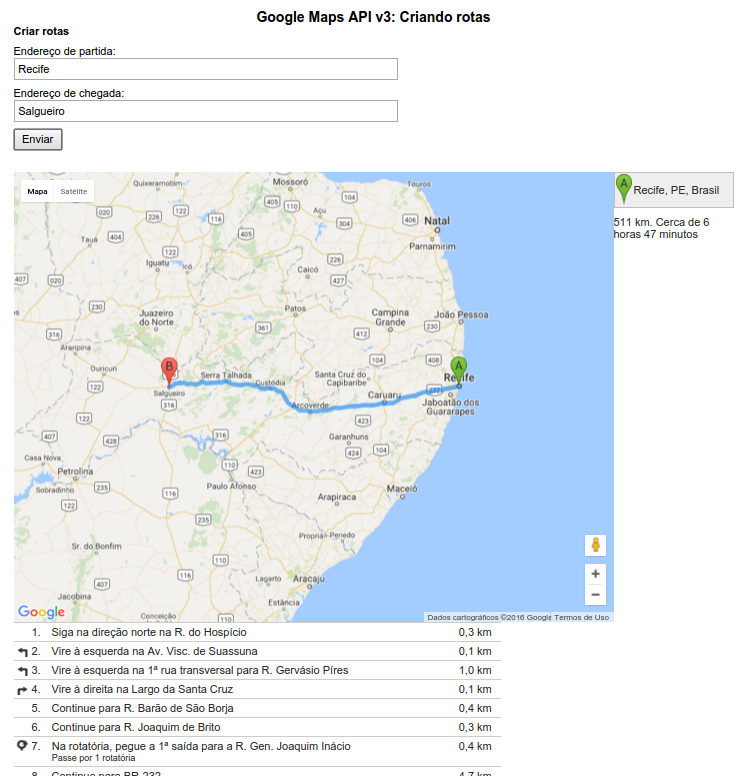
\includegraphics[width=150mm, height=130mm]{Figuras/Cronograma/GoogleMaps.png}
\end{figure}

\pagebreak

\section{Casos de teste do modelo preditivo}